\documentclass[12pt]{article}
\usepackage{fullpage}
\usepackage{latexsym}
\usepackage{color}
\usepackage{listings}
\usepackage{caption}
\usepackage{amsfonts,amsmath,amssymb}
\usepackage{graphicx}
\usepackage{multicol}
\usepackage{etoolbox}   % for booleans and much more`
\usepackage{verbatim} % for the comment environment
\usepackage{enumitem}


%\pagestyle{empty}

% set up solutions environment
\newbool{hidesolutions}
\setbool{hidesolutions}{false}

% new environment
\newenvironment{solution}{}

% set conditional behaviour of environment
\ifbool{hidesolutions}{\AtBeginEnvironment{solution}{\comment}
\AtEndEnvironment{solution}{\endcomment}}{\AtBeginEnvironment{solution}{\begin{quote}}
\AtEndEnvironment{solution}{\end{quote}}}


\lstnewenvironment{algorithm}[1][] %defines the algorithm listing environment
{   
    \lstset{ %this is the stype
        mathescape=true,
        frame=tB,
        numbers=left, 
        numberstyle=\normalsize,
        basicstyle=\normalsize, 
        keywordstyle=\color{black}\bfseries\em,
        keywords={input, output, return, datatype, function, in, if, else, for, while, begin, end}
        numbers=left,
        xleftmargin=.04\textwidth,
    }
}{}

\begin{document}

\begin{center}
{ \Large \bf CMPU-241 -- Analysis of Algorithms (Fall 2018)}\\
  \vspace{.05in}
{\large \bf Vassar College -- Computer Science Department}\\
  \vspace{.05in}
  {\bf Homework \#7 -- \ifbool{hidesolutions}{Due December 11\textsuperscript{th}, 2018}{Matthew Imiolek}\\
 }
  \vspace{.15in}
% NAME:\underline{\ \ \ \ \ \ \ \ \ \ \ \ \ \ \ \ \ \ \ \ \ \ \ \ \ \ \ \ \ \ \ \ \ \ \ \ \ \ \ \ \ \ \ }\\

\end{center}


\begin{enumerate}

\item (20 points) Consider the Dijkstra's single-source shortest paths algorithm we discussed in class. It uses an adjacency-list graph representation and has a worst-case asymptotic running time of $O(|V|T_i + |V|T_{em}+|E|T_{dk})$, where $T_i$ is the time it takes to insert an element into the priority queue, $T_{em}$ is the time it takes to extract the minimum-key element, and $T_{dk}$ is the time it takes to decrease the key of an element in the queue.

What would happen to this asymptotic running time if we were to use an adjacency-matrix representation for the graph? Briefly justify your answer.

\begin{solution}
If we used an adjacency-matrix, the asymptotic run time would always be Θ(|V|^2) , causing the runtime to stay the same when compared to that of an adjacency-list which could change depending on the queue implementation. In an adjacency-matrix, instead of being able to just go through the members adjacent to u and relax and decrease their keys like in an adjacency-list, the program would have to go through each vertex, and check if it was connected to u, then relax and decrease it if it was. However, because of how this is done, that step would take O(|V|) time, multiplied by the O(|V|) time of the while loop it is already in, leading to a Θ(|V|^2). The queue implementation would no longer matter as a queue set up does not cause any portion of the program to run slower than |V|^2, meaning that will always be the limiting run-time segment. On the other hand, in class we showed that depending on the queue implementation, specifically if Dijkstra used a adjacency-list and either a binary min-heap or fibonacci heap, then if the graph was sparse it would run faster than Θ(|V|^2), or slower if it was dense. In the case it used a array queue implementation, they would run in the same amount of time. In the end, an adjacency-matrix implementation would always have a run time of Θ(|V|^2), leading it to be better or worse than an adjacency-list implementation depending on the queue set up.

\end{solution}


\item (20 points) Suppose you are given a weighted, directed graph $G = (V,E)$ and a source vertex $s$. $G$'s edges that are outgoing from $s$ may have negative weights, but all other edges have non-negative weights. Furthermore, there are no negative-weight cycles in the graph.

Will Dijkstra's algorithm be able to find the shortest paths for $G$? Briefly justify your answer. If your answer is negative, please provide a counterexample.

\begin{solution}
Yes, it would be able to find the shortest path. In the case that these specific edges are negative, it is still the case that v.d = δ(s, v), for all v exist in V. To prove this is still true with these potentially negative edges we must show, given the shortest path from s to v, which has u before v on that path, that u is for sure on that path. This means u has to be in S. As the negative weighted edges must come first, for all negative edges (u, v), u would be s. s is always in S, and because they are the first two vertices connected, v.d must equal δ(s, v). This means for all possible negative weighted edges, v.d = δ(s, v), for all v exist in V. We also know none of the other edge weights can be negative, so for all of the vertices after the first ones connected to s they will still work in the same proof given in class, adding all the u’s in in the path to S, and finally v to S, which leads S to equal V, and that all v exist in V. It also means that the algorithm will find the shortest path from those non-s vertices to v (δ(u1, v) = weight (u1,v)), and when these are added to the short paths from s to the first node (δ(s, u1) = weight (s,u1)), you get the correct least weight from s to v, so v.d = δ(s, v). As we just showed how these specific negative edges can exist while maintaining Dijkstra’s correctness, we can say that Dijkstra’s algorithm will still compute the shortest paths from source s.
\end{solution}


\item (15 points) Given a weighted, directed graph $G = (V, E)$ with no negative-weight cycles, and a source node $s$, let $m$ represent the number of edges of the longest (in terms of edge count) path out of the set of shortest (in terms of weight) paths from $s$ to the other nodes in $V$.

Write a modified version of the Bellman-Ford algorithm we saw in class that allows it to terminate in $m + 1$ iterations over the edge set, even if $m$ is a priori unknown.


\begin{solution}
\begin{equation}
BellmanFord(G,w,s)
	InitializeSingleSource(G,s)
	ChangesMade = true
	while changesMade == true
		changesMade = false
		for each (u, v) in G.E
			Relax(u,v,w)

Relax(u,v,w)
	if v.d > u.d + w(u,v)
		v.d = u.d + w(u,v)
		v.p = u
		changesMade = true
\end{equation}
\end{solution}

\item (15 points) Argue that if the parent pointer of the source node ever becomes non-nil during the execution of the Bellman-Ford algorithm, that implies the existence of a negative weight cycle in the graph.

\begin{solution}
This implies the existence of a negative weight cycle because the default distance to the source is 0. In order to find a path shorter than 0 to the source, and thus cause the parent pointer for the source to change from nil, that path must have a negative weight, as that is the only way to get below 0. Since the source is the first node looked at during the execution of the Bellman-Ford algorithm, all shortest paths have it as their first node, thus, this negative weighted path already has the source in it, and there is a cycle following that path. This would then mean the graph has a negative weight cycle, as this path with a negative weight could be continually followed, decreasing the weight of the path each time.

\end{solution}


\item (30 points) Write the complete sequence of $D^{(k)}$ and $P^{(k)}$ matrices that result from running Floyd-Warshall's algorithm on the following graph:

\begin{figure}[h]
\centering
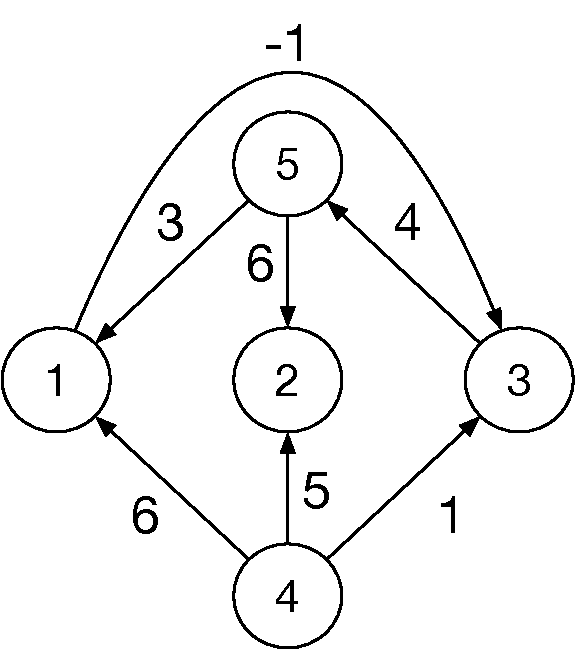
\includegraphics[width=0.28\textwidth]{graph.pdf}
\end{figure}

\begin{solution}
See attached sheet.
\end{solution}

\end{enumerate}

\end{document}



